\documentclass[a4paper, 14pt]{extarticle}

\usepackage[ukrainian]{babel}

\usepackage{fontspec}
\setmainfont{Liberation Serif}

\usepackage{graphicx}
\graphicspath{ {./} }

\usepackage[left=1.18in, right=0.59in, top=0.79in, bottom=0.79in]{geometry}

\usepackage{enumitem}
\usepackage{setspace}
\usepackage{indentfirst}
\usepackage{tocloft}

\usepackage{titlesec}
\titleformat{\section}[block]{\bfseries\filcenter}{}{1em}{}
\titleformat{\subsection}[block]{\bfseries\filcenter}{}{1em}{}

\renewcommand\cfttoctitlefont{\hfill\Large\bfseries}
\renewcommand\cftaftertoctitle{\hfill\mbox{}}

\addto\captionsukrainian{
  \renewcommand\contentsname{ЗМІСТ}
  \renewcommand\refname{ПЕРЕЛІК ДЖЕРЕЛ І ПОСИЛАНЬ}
}

\renewcommand\cftsecdotsep{\cftdot}
\renewcommand\cftsubsecdotsep{\cftdot}
\renewcommand\cftsubsecfont{\normalfont\bfseries}
\renewcommand\cftsubsecpagefont{\normalfont\bfseries}
\renewcommand\cftsubsecleader{\bfseries\cftdotfill{\cftsecdotsep}}

\pagestyle{myheadings}
\setcounter{secnumdepth}{0}

\let\Huge\normalsize
\let\huge\normalsize
\let\LARGE\normalsize
\let\Large\normalsize
\let\large\normalsize

\begin{document}
  \setstretch{1.5}

  \begin{titlepage}
    \begin{center}
      \textbf{КИЇВСЬКИЙ НАЦІОНАЛЬНИЙ УНІВЕРСИТЕТ} \\
      \textbf{ІМЕНІ ТАРАСА ШЕВЧЕНКА} \\
      Факультет комп'ютерних наук та кібернетики \vspace{5em}

      \textbf{Звіт} \\
      за спеціальністю 122 Комп'ютерні науки \\
      на тему: \\
      \textbf{Розробка вебзастосунку для клубу настільних ігор}
    \end{center}
    \vfill
    \begin{flushleft}
      Виконав студент 2-го курсу \\
      Віннічук Назар Дмитрович \vspace{2em}

      Науковий керівник: \\
      доцент, кандидат фіз.-мат. наук \\
      Омельчук Людмила Леонідівна
    \end{flushleft}
    \begin{flushright}
      Засвідчую, що у звіті немає запозичень з \\
      праць інших авторів без відповідних посилань.

      Студент \hspace{7.25em} Віннічук Н. Д.
    \end{flushright}
    \vspace{5em}
    \begin{center}
      Київ -- 2022
    \end{center}
  \end{titlepage}

  \setcounter{page}{2}

  \begin{center}
    \textbf{РЕФЕРАТ}
  \end{center}

  НАСТІЛЬНІ ІГРИ, DJANGO, PYTHON, NIX, POSTGRESQL,
  BOOTSTRAP, ВЕБЗАСТОСУНОК, MVC, ORM.

  Об'єктом роботи є ознайомлення із сучасними вебтехнологіями на базі вебфреймворку
  Django та системою керування базами даних PostgreSQL.

  Предметом роботи є вебзастосунок з реляційною базою даних для забезпечення
  функціонування клубу настільних ігор.

  Метою роботи є створення функціонуючого вебзастосунку для адміністраторів та
  відвідувачів клубу настільних ігор.

  Інструменти розроблення: об'єктно-орієнтована мова програмування Python,
  вебфреймворк Django, система керування базами даних PostgreSQL, мова опису програмних
  пакетів та середовищ розробки Nix, пакетний менеджер Nix,
  мова середовища вебпереглядача JavaScript, мова
  опису структури вебсторінок HTML, мова опису стилів вебсторінок CSS, бібліотека
  готових стилів вебсторінок Bootstrap.

  Результати роботи: розроблено вебзастосунок на основі сучасних вебтехнологій,
  виконано роботу з проектування реляційної бази даних та візуального оформлення
  вебсторінок.

  Програмний продукт здатен використовуватись для реалізації функціонування
  клубу настільних ігор. Вимоги до користувачів: знання української мови (мови
  інтерфейсу застосунку).

  \clearpage
  \setstretch{1}
  \tableofcontents\thispagestyle{myheadings}
  \setstretch{1.5}

  \clearpage
  \section{СКОРОЧЕННЯ ТА УМОВНІ ПОЗНАЧЕННЯ}
  ORM -- Object-Relational Mapping, об'єктно-реляційна відповідність;

  HTML -- HyperText Markup Language, мова розмітки гіпертексту;

  SQL -- Structured Query Language, мова структурованих запитів;

  CSS -- Cascading Style Sheets, таблиці каскадних стилів;

  URL -- Uniform Resource Locator, однорідний вказівник на ресурс.

  \clearpage
  \section{ВСТУП}

  \textbf{Оцінка сучасного стану об'єкта розробки.}
  Ринок програмного забезпечення є наразі наповненим універсальними рішеннями,
  що намагаються покрити велику кількість сфер застосування одним програмним
  продуктом. Проте досі актуальною є потреба в вузькоспеціалізованому програмному
  забезпечені, що виконує лише одну функцію чи покриває лише одну сферу застосування,
  але робить це добре. Таким чином, альтернативні рішення можуть бути універсальнішими
  за наявний предмет розробки, але вони не передбачають вирішення
  для деяких специфічних проблем предметної області.

  \textbf{Актуальність роботи та підстави її виконання.}
  Актуальність роботи полягає в відсутності на ринку програмних продуктів рішень
  для ведення обліку клубів настільних ігор. Такі клуби вже присутні в Україні \cite{igromag},
  тому потреба на такі програмні продукти викликана попитом ринку. Українська мова
  інтерфейсу є іще однією рисою програмного рішення, бажаною для українського ринку.


  \textbf{Мета й завдання роботи.}
  Метою роботи є розробка програмного продукту для застосування адміністраторами
  та гравцями клубу настільних ігор, а також ознайомлення з технологіями, що
  використовуються для розроблення вебзастосунків. Для досягнення мети було поставлено
  такі завдання:

  \begin{enumerate}[nosep, label=\arabic*)]
    \item описати середовище розробки за допомогою мови Nix;
    \item ознайомитися із системою керування базами даних PostgreSQL;
    \item спроєктувати базу даних для предметної області;
    \item створити проєкт вебфреймворку Django та приєднати до нього наявну базу даних;
    \item розробити валідацію моделей предметної області, логіку застосунку та зовнішній
      вигляд представлень.
  \end{enumerate}

  \textbf{Об’єкт, методи й засоби розроблення.}
  Об'єктом розроблення програмного продукту є вебзастосунок, що складається
  з адміністративного інтерфейсу для працівників клубу та зовнішнього інтерфейсу
  для гравців клубу. Адміністративний інтерфейс реалізує додавання, редагування,
  та видалення сутностей предметної області із бази даних застосунку. Серед
  сутностей предметної області є настільні ігри, їх локалізації, автори, ігрові сеанси,
  гравці клубу тощо. Зовнішній інтерфейс для гравців клубу реалізує перегляд наявних
  у клубі настільних ігор, перегляд супутньої до ігор інформації, а також створення
  ігрових сеансів.

  Серед інструментів, використаних для розроблення застосунку, є такі: текстовий редактор
  Vim із розширенням Python Language Server Protocol,
  пакетний менеджер Nix, вбудований командний рядок системи керування базами даних
  PostgreSQL.

  \textbf{Можливі сфери застосування.}
  Програмний продукт може бути використаним клубом настільних ігор, гравці та персонал
  якого володіють українською мовою.

  \clearpage
  \section{РОЗДІЛ 1. ОГЛЯД НАЯВНИХ НА РИНКУ РІШЕНЬ}
  \textbf{Strapi.} Система керування контентом з відкритим кодом.
  Користувач має описати сутності предметної області за допомогою мови JavaScript, після
  чого даний програмний продукт генерує інтерфейс адміністратора для додавання, видалення
  та редагування сутностей. Вбудована підтримка предметної області настільних ігор
  відсутня. Доступ до вебсторінки для перегляду сутностей без можливості видалення та
  редагування потребує створення облікового запису у системі. Можливості зміни вигляду
  вебсторінок обмежені \cite{strapi}.

  \textbf{Joomla.} Система керування контентом з відкритим кодом.
  Користувач має створити сутності предметної області за допомогою графічного
  інтерфейсу адміністративної панелі, після
  чого даний програмний продукт генерує інтерфейс адміністратора для додавання, видалення
  та редагування сутностей. Наявний вбудований конструктор гостьових сторінок.
  Вбудована підтримка предметної області настільних ігор відсутня. Зовнішній вигляд
  вебсторінок та логіка обробки даних може в певних межах бути змінена за допомогою
  графічного інтерфейсу, проте система додатків дозволяє подальшу зміну \cite{joomla}.


  \clearpage
  \section{РОЗДІЛ 2. ОГЛЯД ВИКОРИСТАНИХ ТЕХНОЛОГІЙ}

  \subsection{2.1 Вебфреймворк Django}
  Django -- вебфреймворк високого рівня, що спонукає до швидкої розробки та чистого,
  прагматичного дизайну застосунку. Розробка вебфреймворку здійснюється волонтерами,
  а проєкт має відкритий вихідний код. Розробка вебзастосунків на основі
  вебфреймворку Django здійснюється об'єктно-орієнтованою мовою високого рівня Python.

  Django характеризується наявністю інтегрованих рішень для пересічних завдань
  веброзробки. Серед таких рішень є система автентифікації, ORM, рушій шаблонів HTML,
  та інтерфейс адміністратора, що здатен надати базовий функціонал керуванням
  сутностями предметної області за визначенням ORM моделей \cite{django}.

  \subsection{2.2. Система керування базами даних PostgreSQL}
  Дана система керуванням базами даних позиціонує себе як найрозвиненішу у сфері
  реляційних баз даних. Розробники даної системи високо цінують відповідність стандартам
  мови SQL, проте це не заважає системі мати чисельні нестандартні розширення,
  серед яких типи стовпців JavaScript Object Notation та спадкування таблиць. Іще однією
  перевагою даної системи є вичерпність та зрозумілість офіційної документації.

  За замовчуванням, PostgreSQL працює у режимі глобального встановлення, тобто передбачається
  не більше одного сервера бази даних на одну машину, а файли баз даних зберігаються
  у глобальних системних каталогах. Проте за допомогою нечисельних змін до
  налаштувань, PostgreSQL може працювати локально в межах довільного одного каталогу
  користувача, що робить дану систему керування базами даних зручною в процесі
  розробки \cite{postgres}.

  PostgreSQL сумісний з мовою програмування Python за рахунок бібліотеки Psycopg,
  яка у свою чергу сумісна з Django ORM \cite{psycopg} \cite{django}.

  \subsection{2.3. Пакетний менеджер та мова опису середовищ Nix}
  Nix -- назва пакетного менеджеру, а також мови програмування для опису програмних
  пакетів, з якими цей менеджер працює. Мова Nix повністю декларативна та функціональна.
  Обчислення Nix зазвичай герметичне, тобто один і той же вираз мовою Nix обчислюється в один
  і той же результат незалежно від середовища виконання. Такі властивості дозволяють
  програмним пакетам, зібраним на основі їх опису мовою Nix, працювати на довільній іншій
  системі, де встановлено Nix.

  Бібліотека готових пакетів для пакетного менеджера Nix містить пакети для
  Django, PostgreSQL, Vim тощо. Пакети, відсутні у стандартній бібліотеці, можна
  встановити, описавши їх мовою Nix \cite{nixos}.

  \subsection{2.4. Бібліотека вебстилів Bootstrap}
  Дану бібліотеку було створено компанією Twitter Inc. У ній знаходяться готові
  CSS стилі для застосування до логічних компонентів інтерфейсу, як от
  кнопки та спадні списки. Разом з файлами CSS постачаються файли JavaScript для
  опису логіки поведінки компонентів, проте цей компонент Bootstrap є необов'язковим.
  Стилі Bootstrap можна змінювати та перевикористовувати за допомогою системи CSS змінних
  \cite{bs}.

  \clearpage
  \section{РОЗДІЛ 3. ПРИЗНАЧЕННЯ І ЦІЛІ СТВОРЕННЯ ЗАСТОСУНКУ}

  \subsection{3.1. Призначення застосунку}
  Застосунок призначений для використання клубами настільних ігор для реалізації
  обліку каталогу настільних ігор та зовнішнього інтерфейсу для гравців, що дозволяє
  переглядати каталог та ініціювати ігрові сеанси.

  Робота передбачає:

  \begin{itemize}[nosep]
    \item проєктування реляційної бази даних на основі системи керування
      базами даних PostgreSQL;
    \item освоєння вебфреймворку Django;
    \item реалізацію логіки предметної області;
    \item реалізацію адміністративного інтерфейсу та зовнішнього інтерфейсу користувача.
  \end{itemize}

  \subsection{3.2. Цілі створення застосунку}
  Застосунок створювався з метою:

  \begin{itemize}[nosep]
    \item надання працівникам клубу можливості створювати, змінювати,
      переглядати та видаляти відомості про наявний каталог настільних ігор,
      зарезервовані ігрові сеанси та гравців клубу;
    \item надання дружнього інтерфейсу для гравців клубу з метою перегляду
      наявного каталогу настільних ігор та створення ігрових сеансів.
  \end{itemize}

  \clearpage
  \subsection{3.3. Технічні вимоги}
  Вебпереглядач: Google Chrome версії 50 та вище, Mozilla Firefox версії 50 та вище.

  Операційна система: Linux.

  Розрядність операційної системи: x86-64.

  Встановлене програмне забезпечення: пакетний менеджер Nix.

  У разі помилок введення даних з боку користувача застосунок відповідає інформативними
  повідомленнями про помилку українською мовою. Повідомлення про помилку
  відображаються в межах основного адміністративного чи зовнішнього інтерфейсу вебзастосунку.

  Джерелом даних для застосунку є реляційна база даних на основі системи керування
  базами даних PostgreSQL.
  
  \clearpage
  \section{РОЗДІЛ 4. ОПИС СТРУКТУРИ БАЗИ ДАНИХ}
  Для реалізації функціонування застосунку було спроєктовано реляційну базу
  даних із структурою, що зображена на Рис. \ref{db}. Створення структури
  бази даних у системі PostgreSQL виконувалось мовою SQL за допомогою вбудованого
  командного рядка PostgreSQL.

  \begin{figure}[h]
    \includegraphics[scale=0.39]{figures/db.pdf}
    \centering
    \caption{Діаграма бази даних}
    \label{db}
  \end{figure}

  \clearpage
  \section{РОЗДІЛ 5. РЕАЛІЗАЦІЯ ЗАСТОСУНКУ}
  \subsection{5.1. Опис програмного середовища та залежностей проєкту}
  Задля встановлення необхідних для застосунку програмних залежностей було
  створено файл flake.nix, у якому знаходиться вираз мовою Nix і за яким
  однойменний пакетний менеджер здатен встановити залежності. Серед вже
  існуючих у стандартній бібліотеці пакетів було встановлено:

  \begin{itemize}[nosep]
    \item Python
    \item Django
    \item PostgreSQL
    \item Psycopg
    \item Django-Tables
  \end{itemize}

  Задля полегшення роботи з бібліотекою Bootstrap у вебфреймворці Django
  було самостійно описано та встановлено пакет для Django-Bootstrap.


  \subsection{5.2. Створення моделей}
  Задля початкової генерації Django ORM моделей на основі існуючої бази даних було
  використано офіційний скрипт мовою Python на ім'я inspectdb
  від спільноти розробників Django. Згенеровані таким чином моделі у підсумку зазнали
  наступних змін:

  \begin{itemize}[nosep]
    \item додавання правил валідації відповідно до предметної області;
    \item визначення каскадного видалення як поведінки за замовчуванням
      під час спроби видалення сутності, на які посилаються інші сутності;
    \item додавання україномовних метаданих до моделей та їх атрибутів.
  \end{itemize}

  \subsection{5.3. Створення контролерів}
  Спочатку до Django проєкту було додано контролери адміністрування, що обробляли запити
  за URL, що починались з префіксу /admin. Контролери використовували самостійно розроблені,
  нестандартні форми, що поліпшували інтерфейс у порівнянні з готовими рішеннями.
  Надалі було додано контролери для зовнішнього інтерфейсу, що обробляли запити до решти
  URL.

  \subsection{5.4. Створення зовнішнього інтерфейсу}
  Зовнішній інтерфейс було створено за допомогою вбудованого в Django рушія HTML шаблонів.
  Для стилізації було використано як готові стилі з бібліотеки Bootstrap, так і власні
  стилі. За допомогою бібліотеки Google Charts було створено два кругові графіки, що
  відображали дані про каталог настільних ігор на головній сторінці у режимі реального часу.

  \clearpage
  \section{РОЗДІЛ 6. ІНСТРУКЦІЯ КОРИСТУВАЧА}
  Початкова сторінка для гравців клубу знаходиться за URL / (Рис. \ref{index}).
  На цій сторінці гравець може
  переглянути поточний каталог, за бажанням відсортувавши його за різними стовпцями.
  У лівому верхньому куті початкової та інших сторінок зовнішнього інтерфейс наявна
  довідка.

  \begin{figure}[h]
    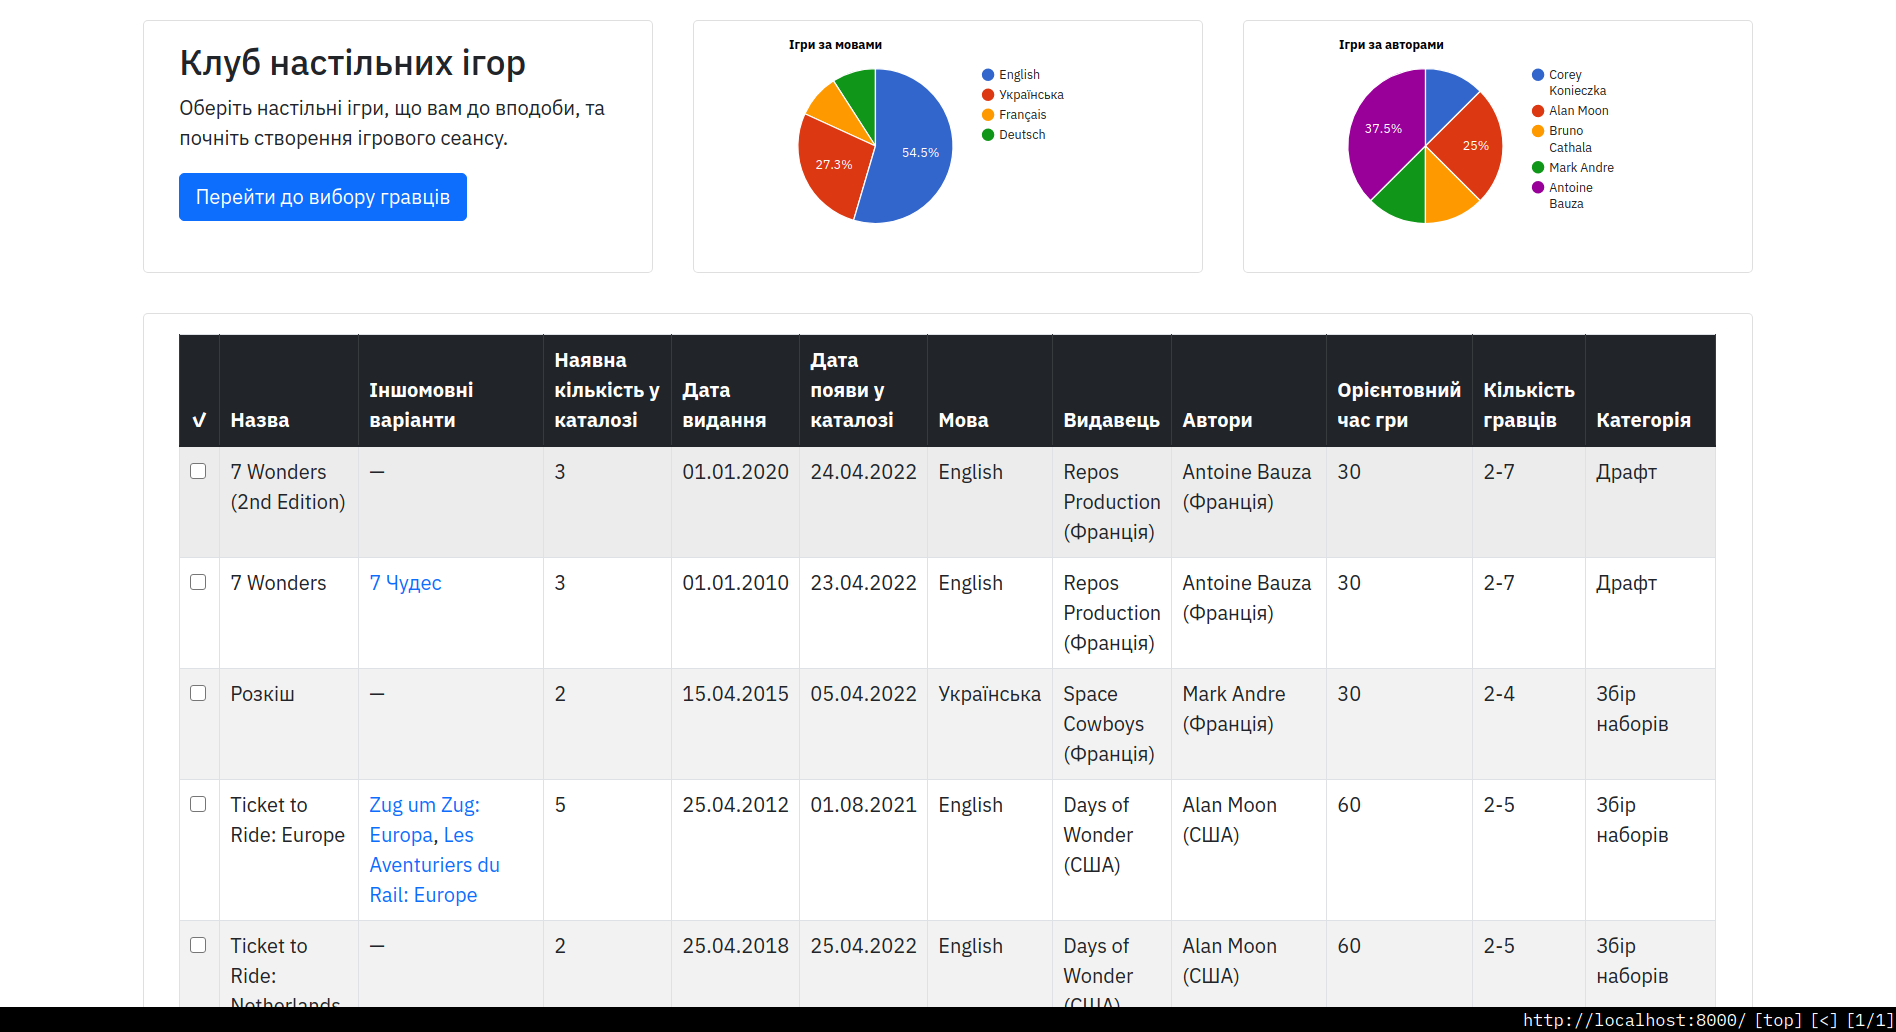
\includegraphics[width=\textwidth]{figures/index.png}
    \centering
    \caption{Початкова сторінка}
    \label{index}
  \end{figure}

  Обравши на головній сторінці бажані ігри, гравець може перейти до наступних форм
  (Рис. \ref{players}, Рис. \ref{time}) та завершити створення сеансу.

  \begin{figure}[h]
    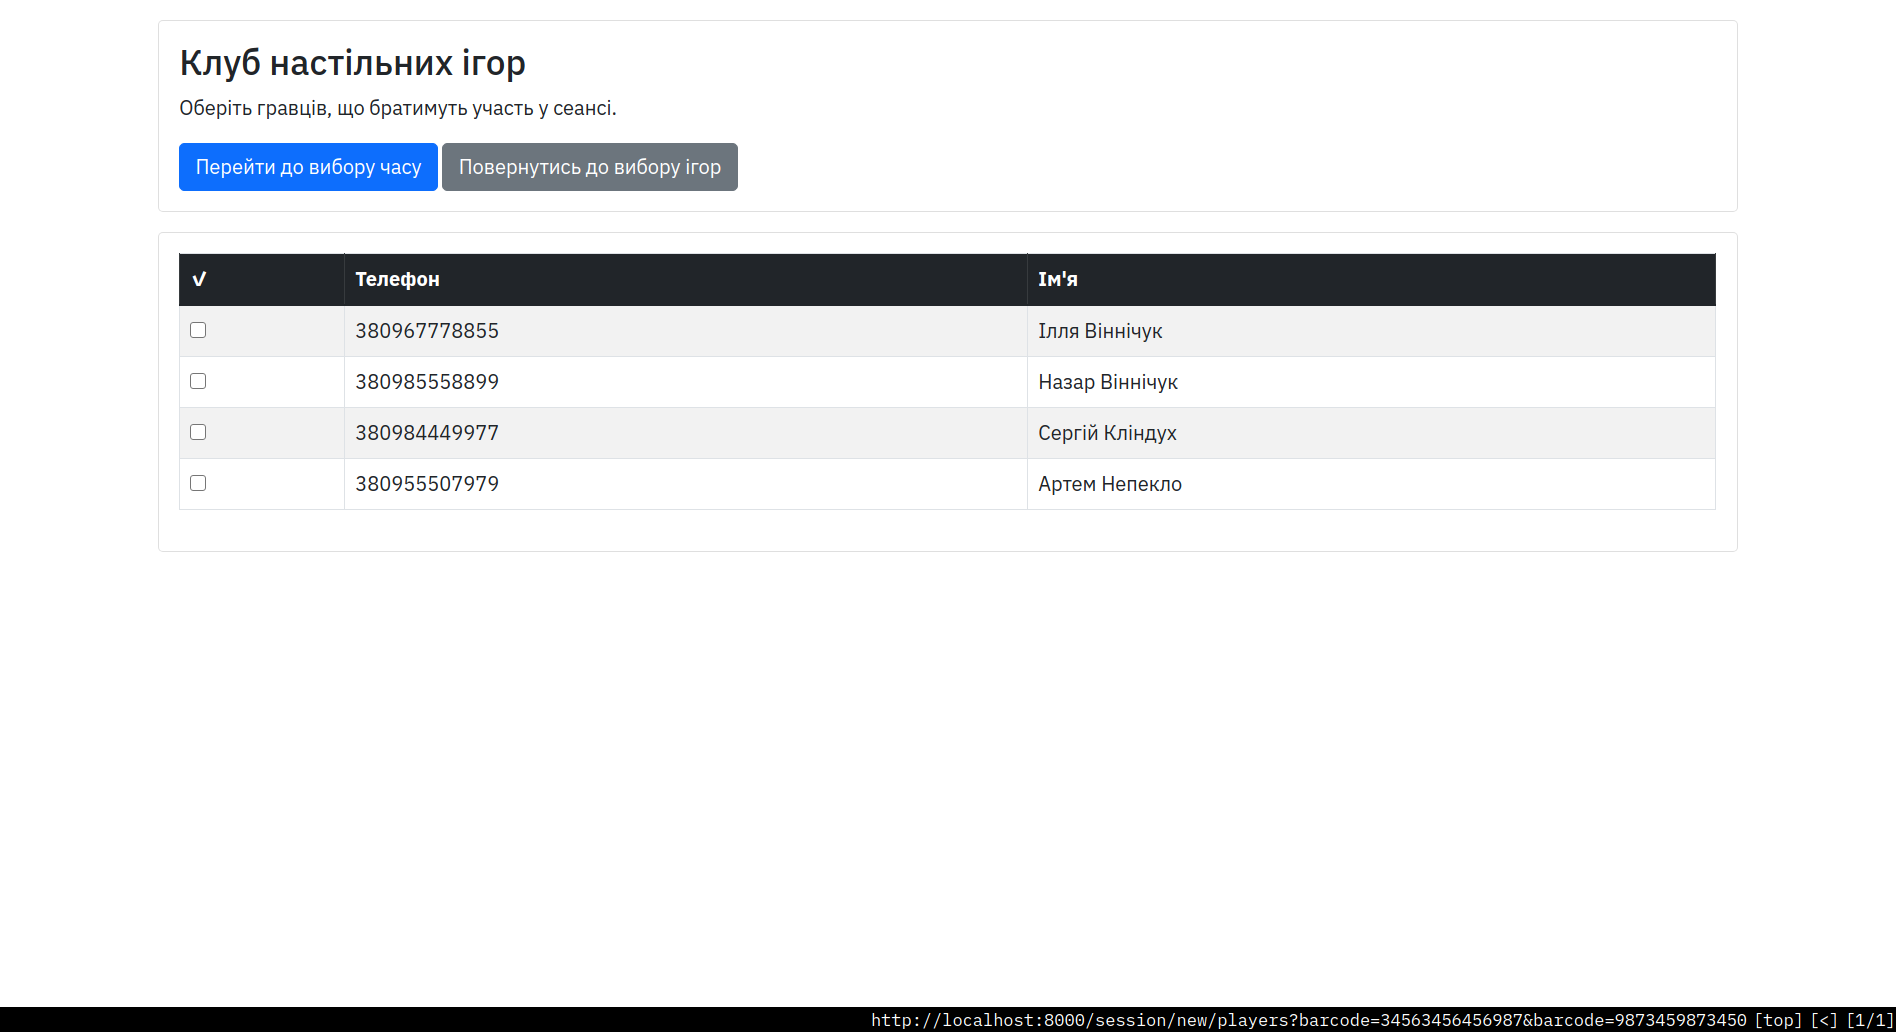
\includegraphics[width=\textwidth]{figures/players.png}
    \centering
    \caption{Форма вибору гравців}
    \label{players}
  \end{figure}

  \begin{figure}[h]
    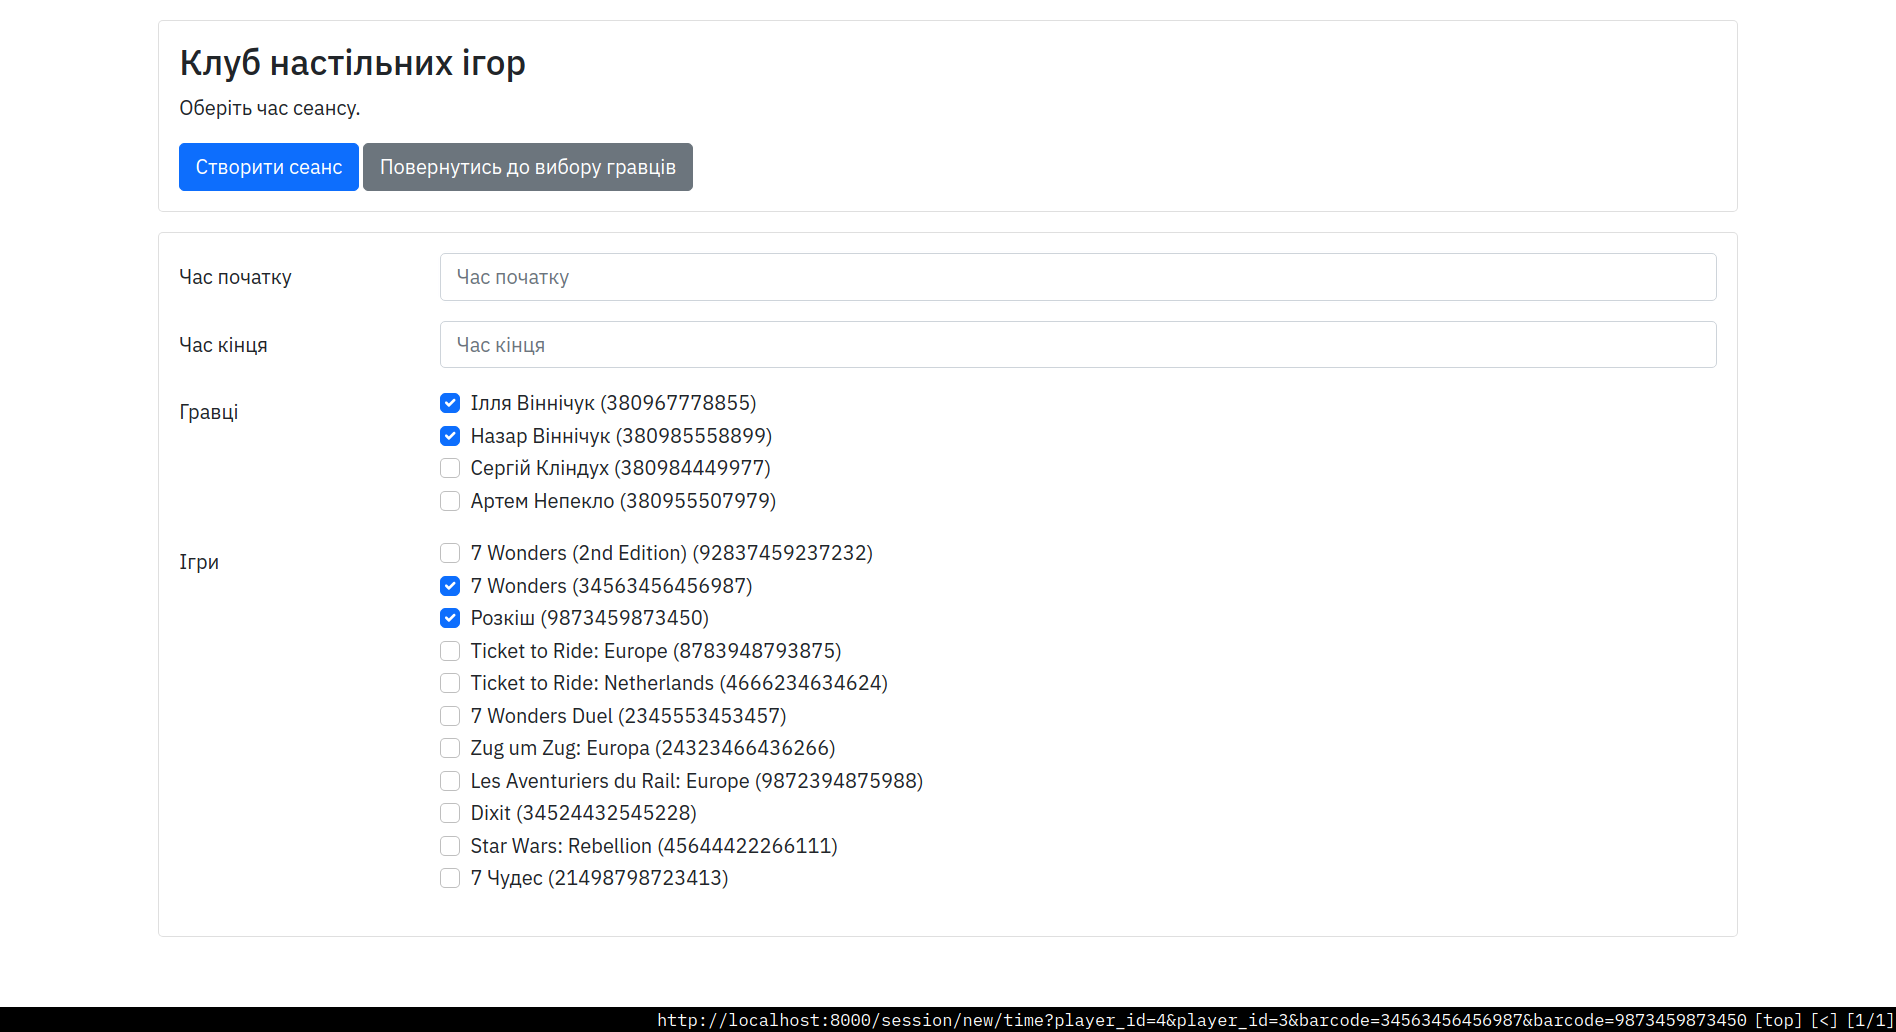
\includegraphics[width=\textwidth]{figures/time.png}
    \centering
    \caption{Форма вибору часу та створення сеансу}
    \label{time}
  \end{figure}

  Адміністративний інтерфейс має сторінки переліку сутностей (Рис. \ref{plp}) та
  сторінки редагування сутностей (Рис. \ref{pdp}).

  \begin{figure}[h]
    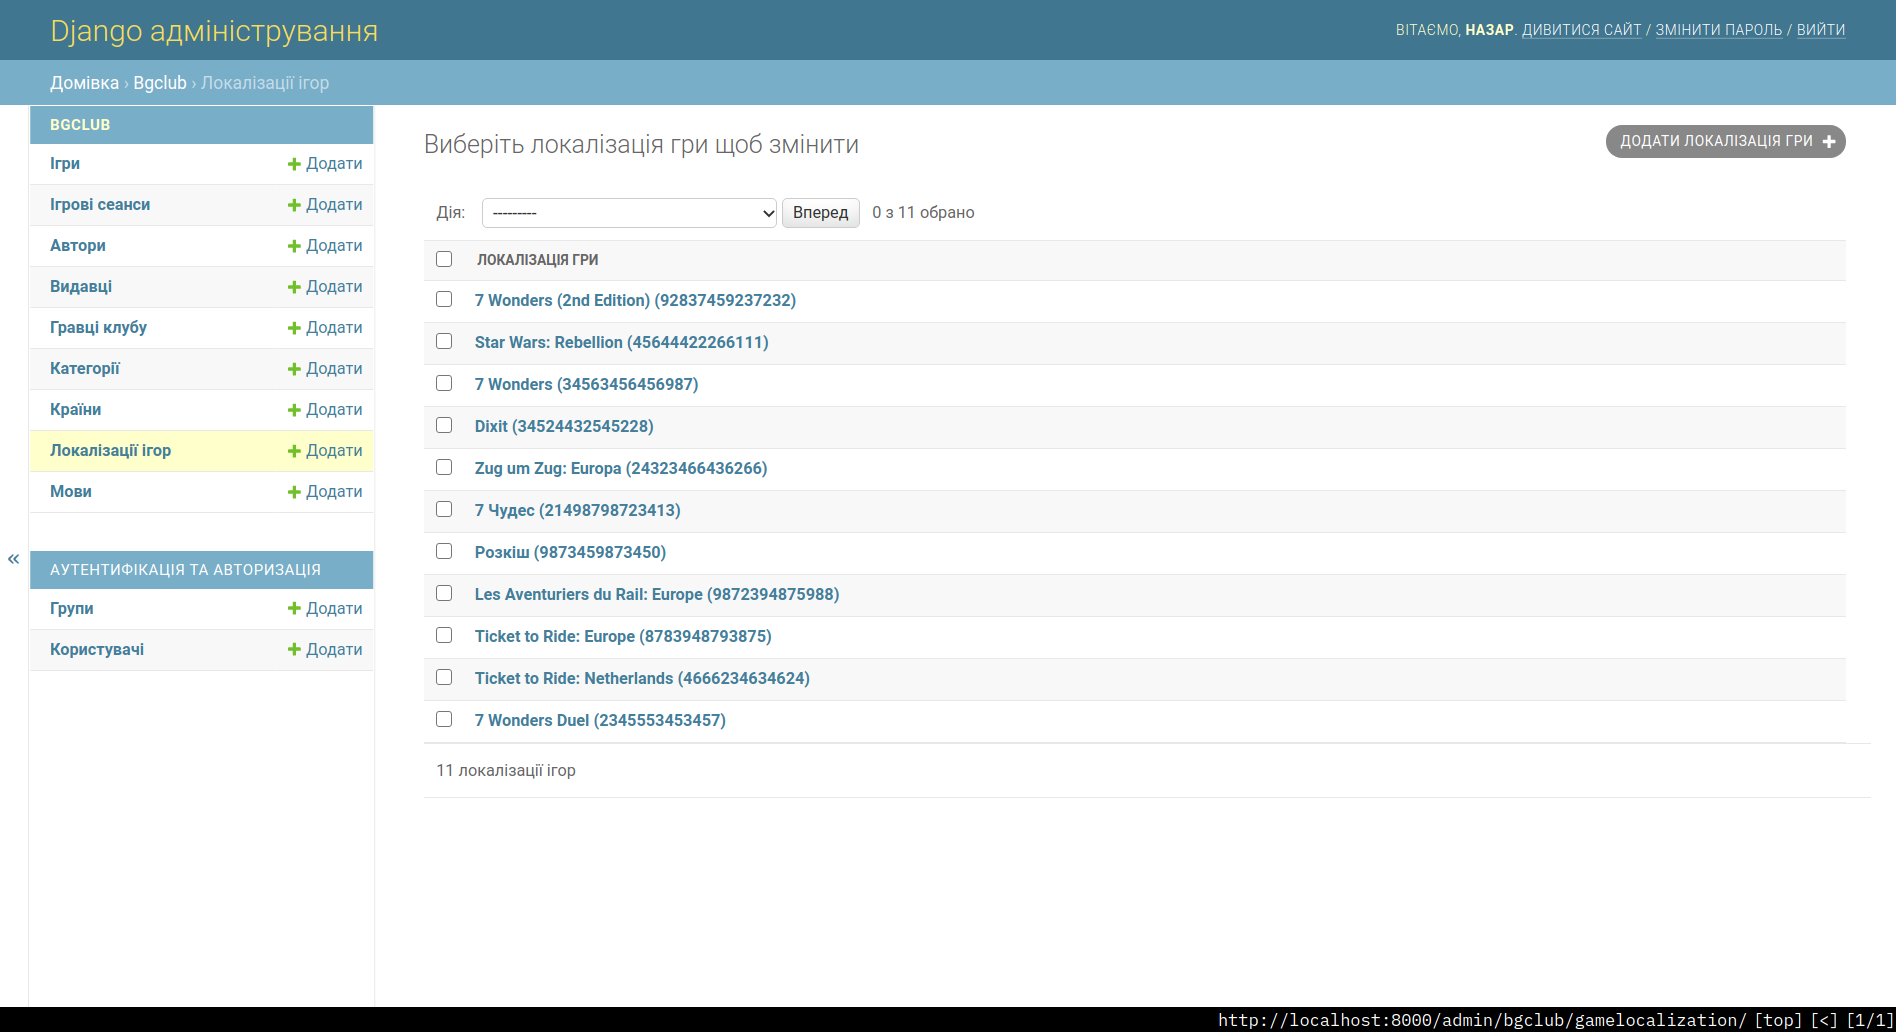
\includegraphics[width=\textwidth]{figures/plp.png}
    \centering
    \caption{Перелік сутностей}
    \label{plp}
  \end{figure}

  \begin{figure}[h]
    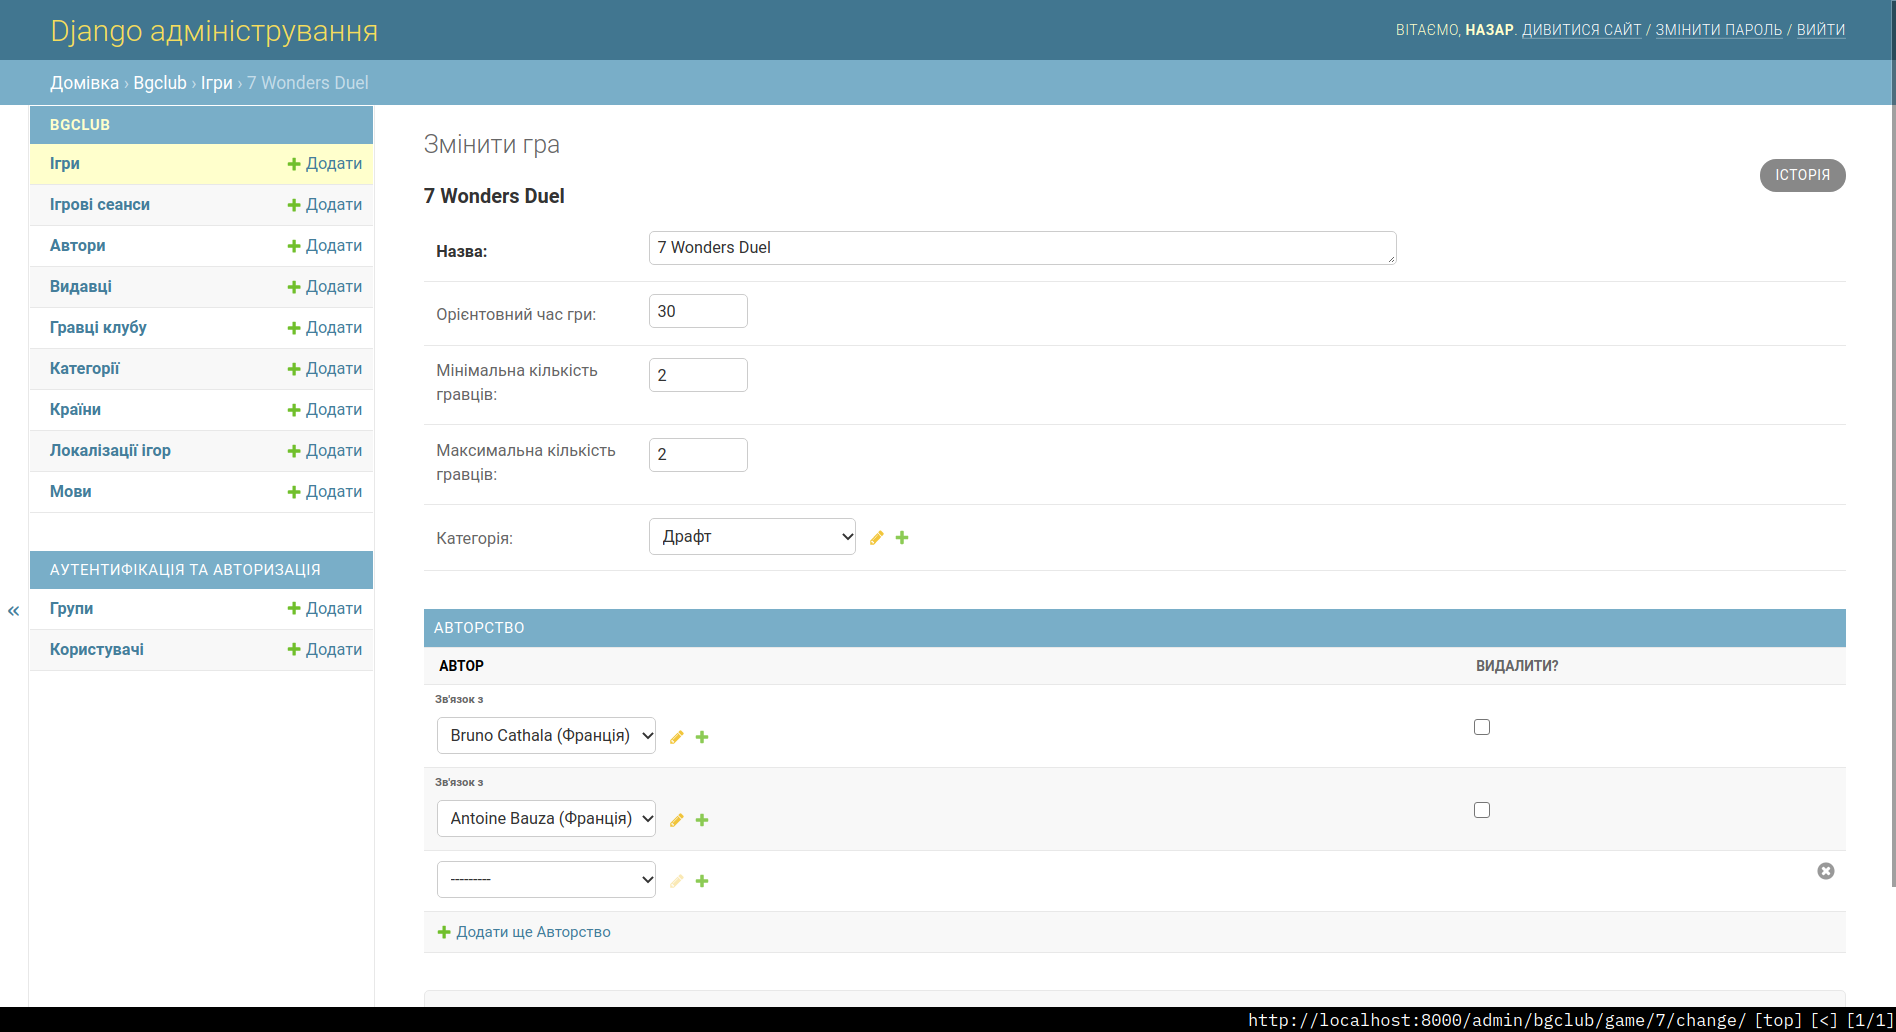
\includegraphics[width=\textwidth]{figures/pdp.png}
    \centering
    \caption{Редагування сутності}
    \label{pdp}
  \end{figure}

  \clearpage
  \section{ВИСНОВКИ}
  Результатом виконаної роботи є функціонуючий вебзастосунок, що задовольняє вимоги предметної
  області. Застосунок надає користувацький інтерфейс як для працівників клубу наступних
  ігор, так і для його відвідувачів. Запорукою успішної реалізації проєкту стали обрані
  технології: Python, Django, PostgreSQL, Nix, Bootstrap. Вони надавали можливість
  процесу розробки бути водночас швидким, легким та приємним, а архітектурі застосунку
  бути чіткою та зрозумілою.

  Іще одним результатом даної роботи стало ознайомлення з технологіями для
  розробки вебзастосунків: як з деталями обраних технологій, так і із загальними принципами,
  що застосовні до сфери загалом.

  \clearpage
  \addcontentsline{toc}{section}{ПЕРЕЛІК ДЖЕРЕЛ І ПОСИЛАНЬ}
  \begin{thebibliography}{9}
    \bibitem{igromag} Клуб настільних ігор Ігромаг [Електронний ресурс]
    -- Режим доступу до ресурсу:
    https://igromag.club/

    \bibitem{strapi} Strapi CMS [Електронний ресурс] -- Режим доступу до ресурсу:
    https://strapi.io/

    \bibitem{joomla} Joomla CMS [Електронний ресурс] -- Режим доступу до ресурсу:
    https://docs.joomla.org/

    \bibitem{django} Django [Електронний ресурс] -- Режим доступу до ресурсу:
    https://www.djangoproject.com/

    \bibitem{postgres} PostgreSQL [Електронний ресурс] -- Режим доступу до ресурсу:
    https://www.postgresql.org/

    \bibitem{psycopg} Psycopg [Електронний ресурс] -- Режим доступу до ресурсу:
    https://www.psycopg.org/

    \bibitem{nixos} Nix [Електронний ресурс] -- Режим доступу до ресурсу:
    https://nixos.org/

    \bibitem{bs} Bootstrap [Електронний ресурс] -- Режим доступу до ресурсу:
    https://getbootstrap.com/

  \end{thebibliography}

\end{document}
